
\section{Experiments}
\label{sec:exp}

%   We use LSTM \addref implementation of RNN and ELU \addref nonlinearities unless stated otherwise.

  \subsection{KTH Pedestrian Tracking}
      
	\begin{figure}
		\centering
		\begin{tikzpicture}
		    \draw[->] (0, 0) -- node[above] {\small time} (10, 0);
		\end{tikzpicture}
		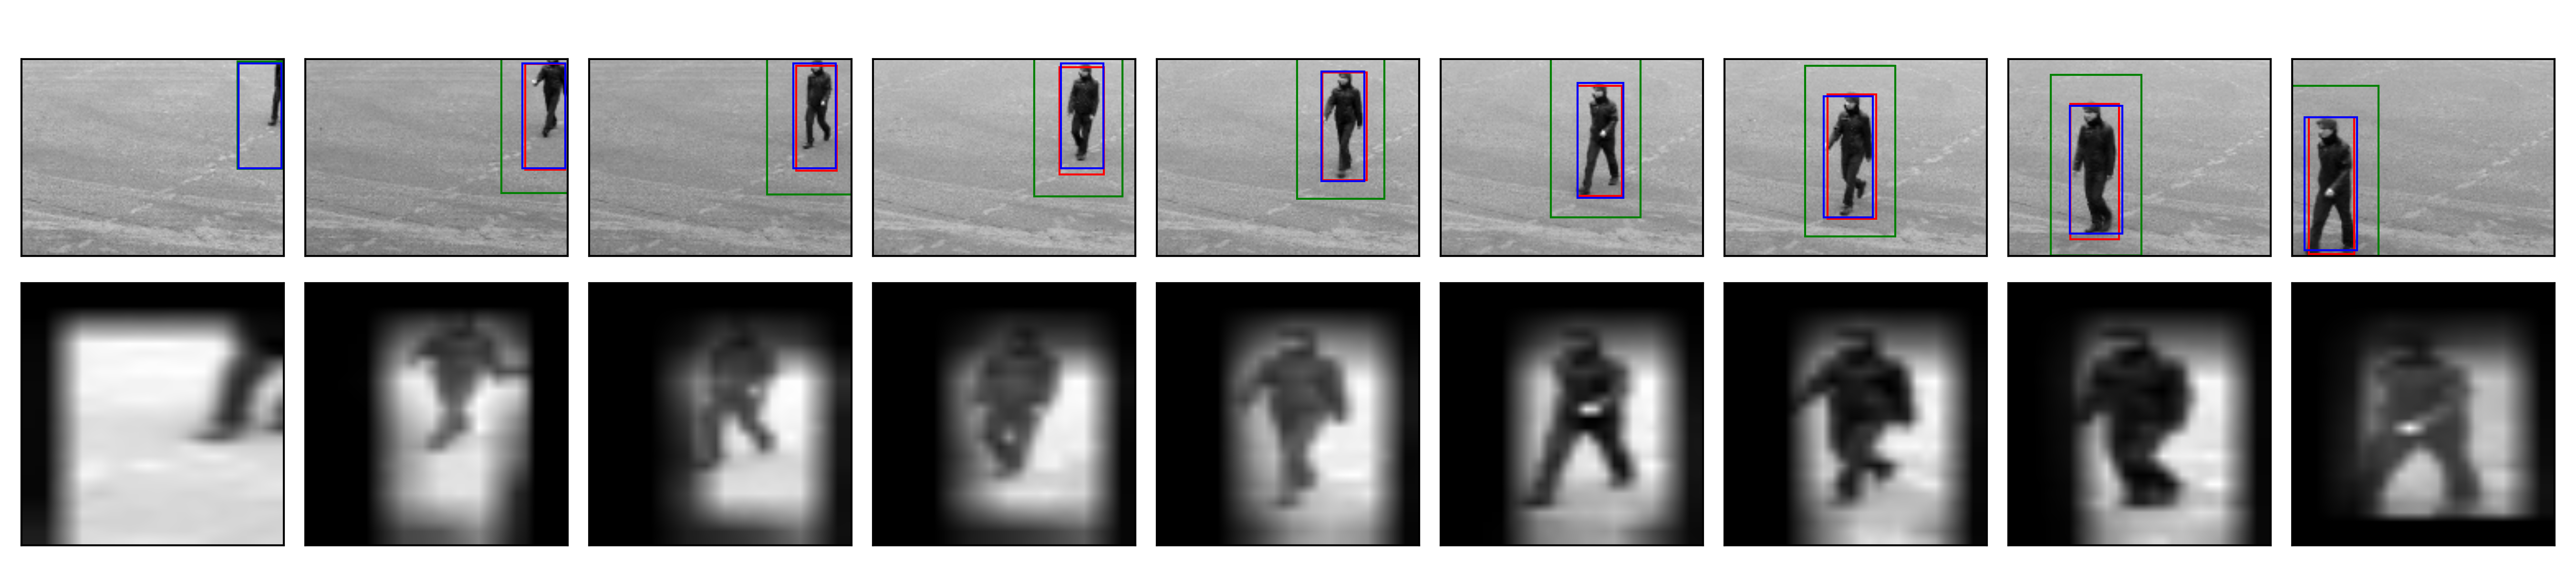
\includegraphics[width=\textwidth]{HART/kth_overlay_16}
		\caption{Tracking results on KTH dataset \cite{KTH_activity_recognition}. Starting with the first initialisation frame where all three boxes overlap exactly, time flows from left to right showing every $16^{th}$ frame of the sequence captured at 25fps. The colour coding follows from  \Cref{fig:img_with_att}. The second row shows attention glimpses multiplied with appearance attention.}
		\label{fig:kth}
	\end{figure}

    \citet{Kahou2015ratm} performed a pedestrian tracking experiment on the KTH activity recognition dataset \cite{KTH_activity_recognition} as a real-world case-study. We replicate this experiment for comparison. We use code provided by the authors for data preparation and we also use their pre-trained feature extractor. Unlike them, we did not need to upscale ground-truth bounding boxes by a factor of 1.5 and then downscale them again for evaluation. We follow the authors and set the glimpse size $\fences{h, w} = \fences{28, 28}$. We replicate the training procedure exactly, with the exception of using the RMSProp optimiser \cite{Hinton2015RMSProp} with learning rate of $3.33 \times 10^{-5}$ and momentum set to $0.9$ instead of the stochastic gradient descent with momentum. The original work reported an IoU of 55.03\% on average, on test data, while the presented work achieves an average IoU score of 77.11\%, reducing the relative error by almost a factor of two. \Cref{fig:kth} presents qualitative results.
    
  \subsection{Scaling to Real-World Data: KITTI}
	
% 
\begin{table}
    % \hfill
    \begin{minipage}[r]{0.6\linewidth}
        \centering
	   % \todo[inline]{other results are on their way}
	    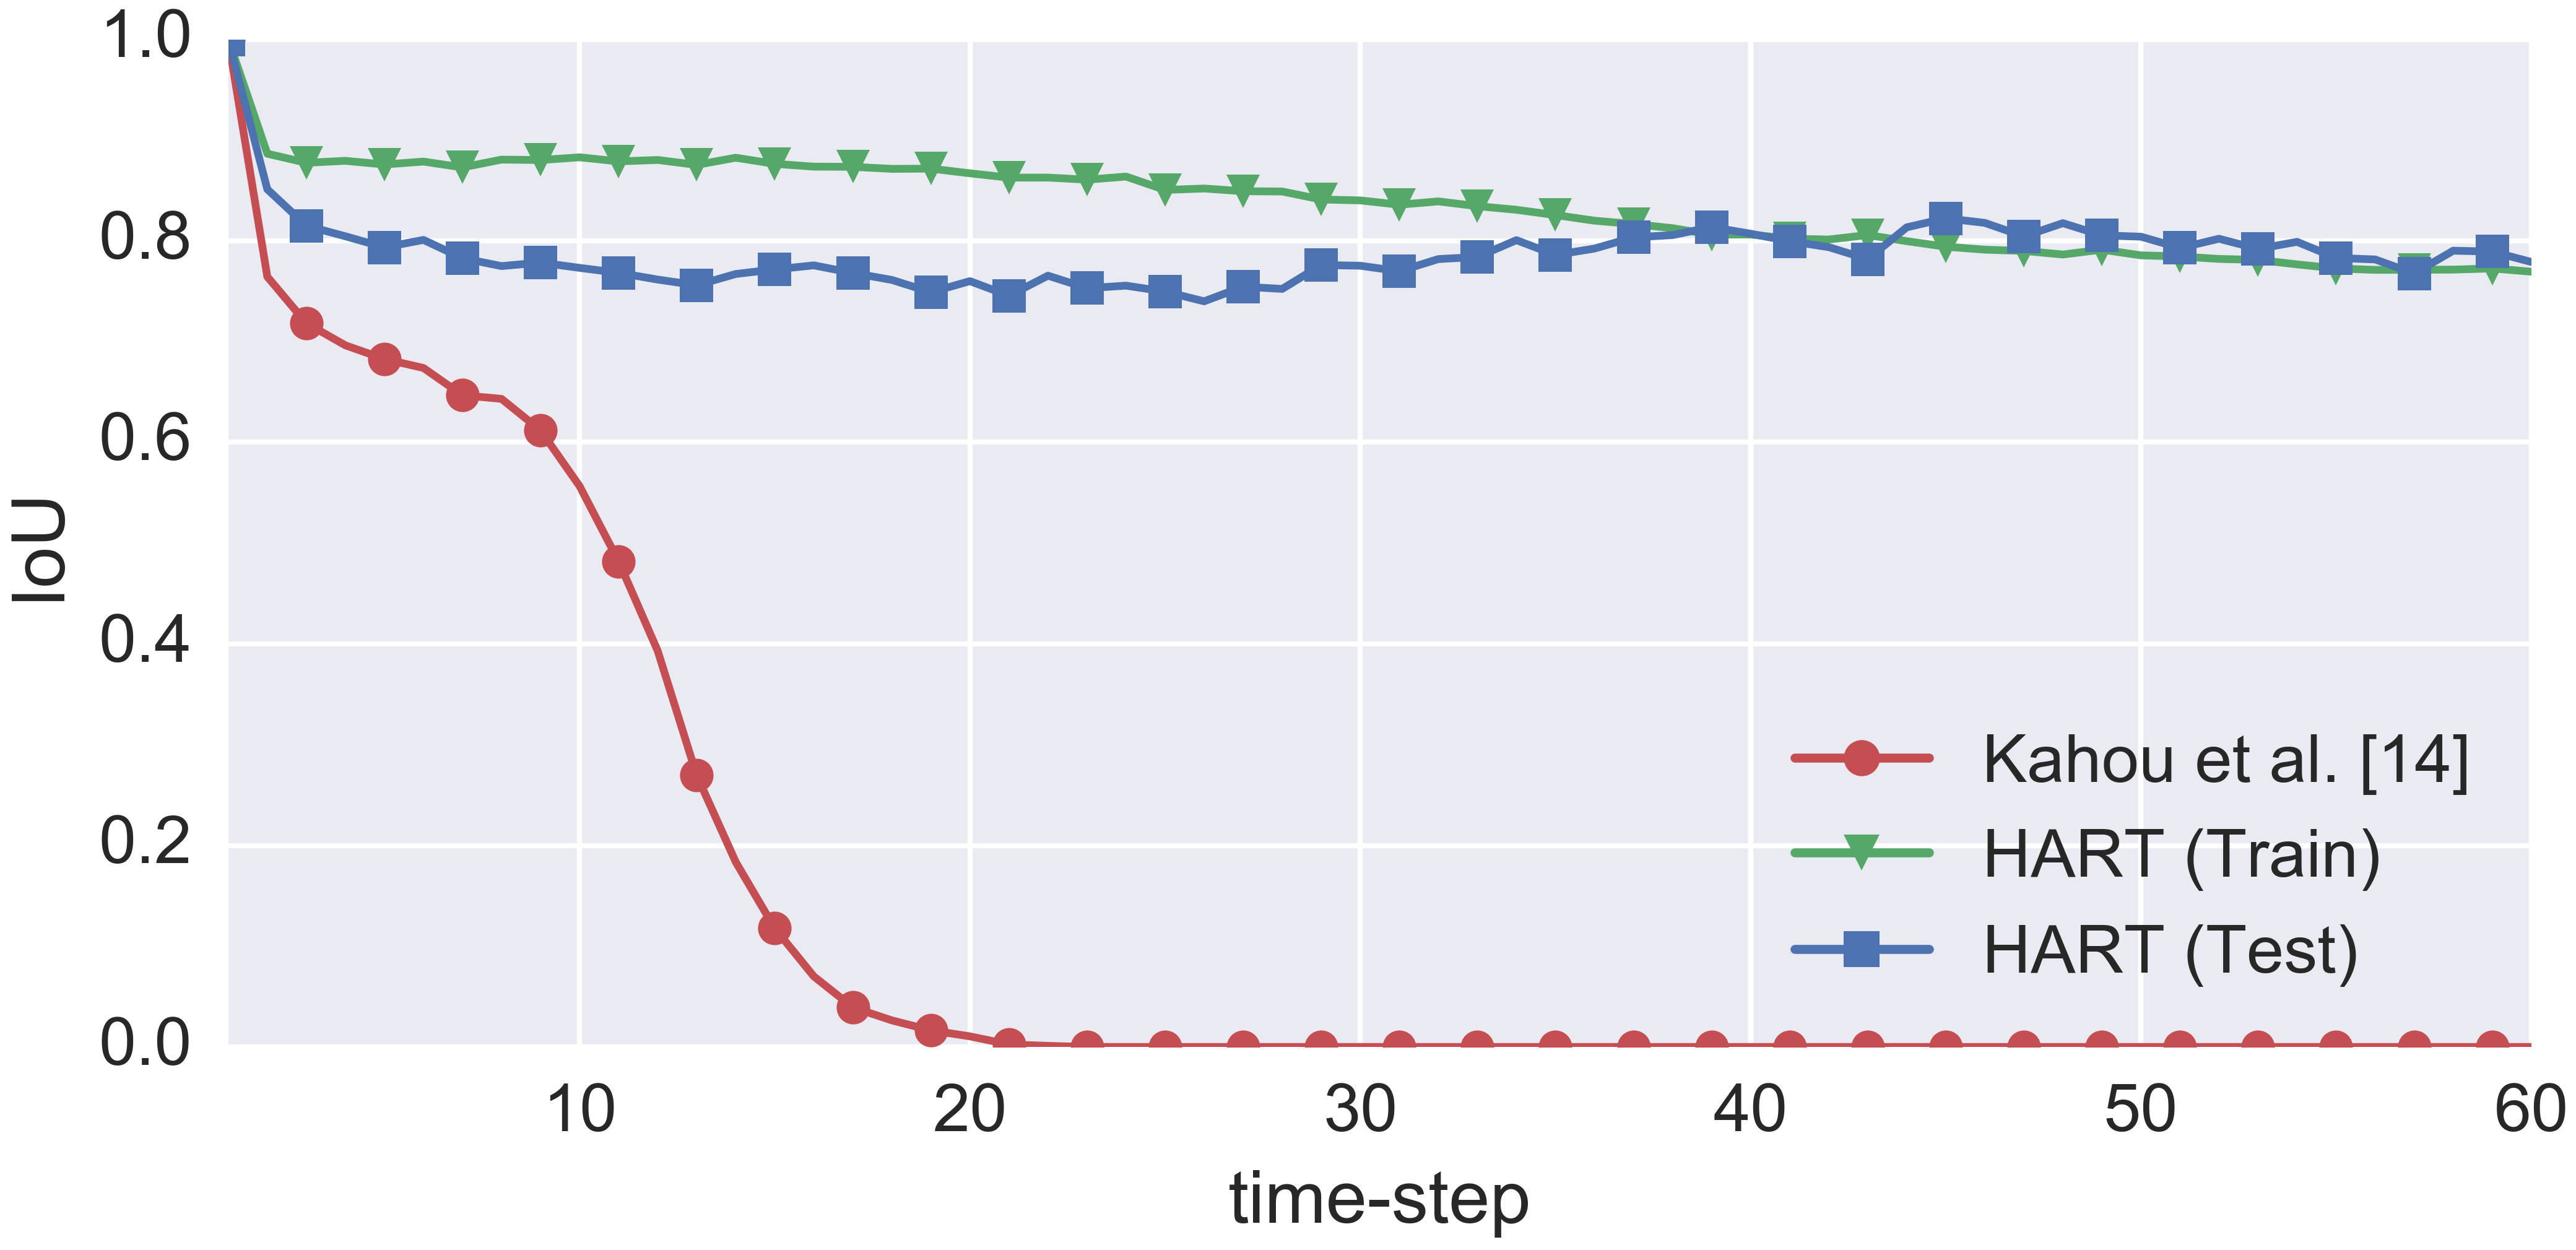
\includegraphics[width=\textwidth]{HART/kitti_iou_fig}
	    \captionof{figure}{IoU curves on KITTI over 60 timesteps. HART (train) presents evaluation on the train set (we do not overfit).}
	    \label{fig:kitti_iou_fig}
    \end{minipage}
    \hfill
    \begin{minipage}[t]{0.35\linewidth}
    	\centering
    	 \begin{tabular}{c|c}
    		\toprule
    		Method                      &   Avg. IoU\\
    		\midrule
    		\citet{Kahou2015ratm}       &   0.14      \\
    		Spatial Att                 &   0.60       \\  
    % 			Spatial Att with Loss       &   0.70   \\
    		App Att                     &   0.78       \\
    		HART                        &   \B{0.81}   \\
    		\bottomrule
    	\end{tabular}
    	\caption{Average IoU on KITTI over 60 time-steps.}
    	\label{tab:kitti}
    \end{minipage}
\end{table}

    Since we demonstrated that pedestrian tracking is feasible using the proposed architecture, we proceed to evaluate our model in a more challenging multi-class scenario on the KITTI dataset \cite{Geiger2013}. It consists of 21 high resolution video sequences with multiple instances of the same class posing as potential distractors. We split all sequences into 80/20 sequences for train and test sets, respectively. As images in this dataset are much more varied, we implement V1 as the first three convolutional layers of a modified AlexNet \cite{Krizhevsky2012}. The original AlexNet takes inputs of size $227 \times 227$ and downsizes them to $14 \times 14$ after \emph{conv3} layer. Since too low resolution would result in low tracking performance, and we did not want to upsample the extracted glimpse, we decided to replace the initial stride of four with one and to skip one of the max-pooling operations to conserve spatial dimensions. This way, our feature map has the size of $14 \times 14 \times 384$ with the input glimpse of size $\fences{h, w} = \fences{56, 56}$. We apply dropout with probability 0.25 at the end of V1. The ventral stream is comprised of a single convolutional layer with a $1 \times 1$ kernel and five output feature maps. The dorsal stream has two dynamic filter layers with kernels of size $1 \times 1$ and $3 \times 3$, respectively and five feature maps each. We used 100 hidden units in the RNN with orthogonal initialisation and Zoneout \cite{Krueger2016} with probability set to 0.05. The system was trained via curriculum learning \cite{Bengio2009}, by starting with sequences of length five and increasing sequence length every 13 epochs, with epoch length decreasing with increasing sequence length. We used the same optimisation settings, with the exception of the learning rate, which we set to $3.33 \times 10^{-6}$.
    
    
    \Cref{tab:kitti} and \Cref{fig:kitti_iou_fig} contain results of different variants of our model and of the RATM tracker by \citet{Kahou2015ratm} related works. \emph{Spatial Att} does not use appearance attention, nor loss on attention parameters. \emph{App Att} does not apply any loss on appearance attention, while \emph{HART} uses all described modules; it is also our biggest model with 1.8 million parameters. Qualitative results in the form of a video with bounding boxes and attention are available online \footnote{\url{https://youtu.be/Vvkjm0FRGSs}}. We implemented the RATM tracker of \citet{Kahou2015ratm} and trained with the same hyperparameters as our framework, since both are closely related. It failed to learn even with the initial curriculum of five time-steps, as RATM cannot integrate the frame $\bxt$ into the estimate of $\bbt$ (it predicts location at the next time-step). Furthermore, it uses feature-space distance between ground-truth and predicted attention glimpses as the error measure, which is insufficient on a dataset with rich backgrounds. It did better when we initialised its feature extractor with weights of our trained model but, despite passing a few stags of the curriculum, it achieved very poor final performance. 
    
    % We also evaluate the pre-trained models provided by \citet{Valmadre2017cfnn}\footnote{The two layer variant.} and \citet{Savarese2016goturn}, which achieve state-of-the-art performance on the OTB-100 benchmark \cite{OTB}. They do not do well on KITTI, nonetheless. Qualitative evaluation showed rapid and stark scale changes in KITTI sequences as a plausible cause. OTB uses a higher frame rate of 25fps (10fps on KITTI), which leads to relatively smooth scale transitions. To substantiate this case, we trained our tracker on ImageNet Vid dataset \cite{ILSVRC15}, which both \cite{Valmadre2017cfnn,Savarese2016goturn} use for training, and tested on KITTI, which resulted in poor performance.
    
     % \subsection{Scaling to Large Amounts of Data}
    % To test how our framework scales with increasing amount of data we train it on the ImageNet Video dataset \cite{ILSVRC15} and evaluate it on the OTB-50 dataset. We use the same feature extractor and optimisation settings as for the KITTI experiment, but we increase the number of the output feature maps of the ventral stream from five to 20 and the number of neurons of the RNN and all fully-connected layers from 100 to 200, thereby increasing the model size almost twofold, to 3 million parameters. 